\documentclass[tikz]{standalone}
\usepackage{tikz}
\usetikzlibrary{decorations.markings}

\begin{document}

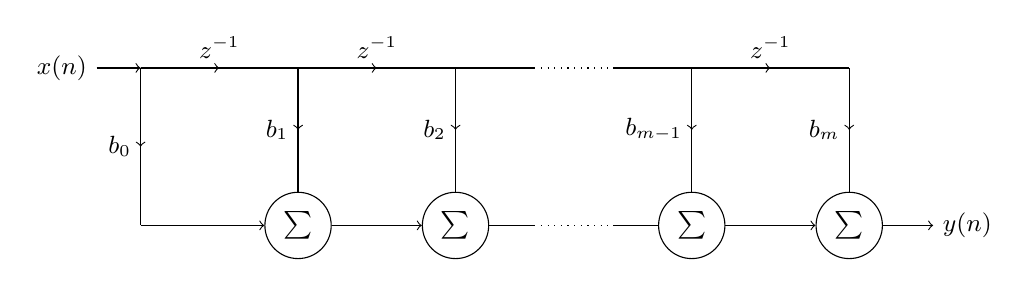
\begin{tikzpicture}[font=\small]
    \tikzset{
        zdelay/.style={
            postaction={decorate},
            decoration={
                markings,
                mark=at position 0.5 with {
                    \arrow{>};
                    \node[above]{$z^{-1}$};
                }
            }
        },
        bgain/.style={
            postaction={decorate},
            decoration={
                markings,
                mark=at position 0.5 with {
                    \arrow{>};
                    \node[left]{#1};
                }
            }
        }
    }

    \node (x) at (0,0) [left]{$x(n)$};
    \coordinate (x0) at ([xshift=1cm] x);
    \coordinate (x1) at ([xshift=2cm] x0);
    \coordinate (x2) at ([xshift=2cm] x1);
    \coordinate (xm1) at ([xshift=3cm] x2);
    \coordinate (xm) at ([xshift=2cm] xm1);
    \coordinate (s0) at ([yshift=-2cm] x0);
    \node[circle,draw] (s1) at ([yshift=-2cm] x1) {$\sum$};
    \node[circle,draw] (s2) at ([yshift=-2cm] x2) {$\sum$};
    \node[circle,draw] (sm1) at ([yshift=-2cm] xm1) {$\sum$};
    \node[circle,draw] (sm) at ([yshift=-2cm] xm) {$\sum$};
    \node (y) at ([xshift=1.5cm] sm) {$y(n)$};

    \draw[->] (x) -- (x0);
    \draw[zdelay] (x0) --  (x1);
    \draw (x2) -- ([xshift=1cm] x2);
    \draw[dotted] ([xshift=1cm] x2) -- ([xshift=-1cm] xm1);
    \draw ([xshift=-1cm] xm1) -- (xm1);
    \draw[zdelay] (x1) -- (x2);
    \draw[zdelay] (xm1) -- (xm);
    \draw[->] (s0) -- (s1);
    \draw[->] (s1) -- (s2);
    \draw[-] (s2) -- ([xshift=1cm] s2.center);
    \draw[dotted] ([xshift=1cm] s2.center) -- ([xshift=-1cm] sm1.center);
    \draw ([xshift=-1cm] sm1.center) -- (sm1);
    \draw[->] (sm1) -- (sm);
    \draw[->] (sm) -- (y);
    \draw[bgain={$b_{0}$}] (x0) -- (s0);
    \draw[bgain={$b_{1}$}] (x1) -- (s1);
    \draw[bgain={$b_{2}$}] (x2) -- (s2);
    \draw[bgain={$b_{m-1}$}] (xm1) -- (sm1);
    \draw[bgain={$b_{m}$}] (xm) -- (sm);
\end{tikzpicture}

\end{document}